% Sketch output, version 0.3 (build 7d, Sun Mar 20 14:11:05 2016)
% Output language: PGF/TikZ,LaTeX
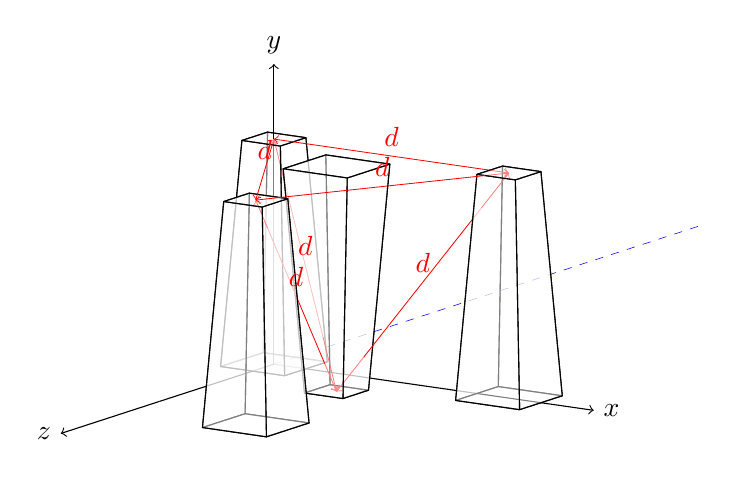
\begin{tikzpicture}[line join=round]
\draw[line width=.2pt,draw=blue,dashed](-2.437,-.792)--(2.708,.88);
\filldraw[fill opacity=0.5,fill=white](-2.031,-.85)--(-2.843,-.733)--(-2.789,2.067)--(-2.302,1.997)--cycle;
\filldraw[fill opacity=0.5,fill=white](-2.843,-.733)--(-3.385,-.909)--(-3.114,1.962)--(-2.789,2.067)--cycle;
\draw[line width=.2pt,draw=blue,dashed](-2.708,-.88)--(-2.437,-.792);
\draw[arrows=-](-2.708,-.88)--(-2.302,-.938);
\filldraw[fill opacity=0.5,fill=white](-2.843,-.733)--(-3.385,-.909)--(-2.572,-1.026)--(-2.031,-.85)--cycle;
\draw[line width=.3pt,arrows=->,draw=red](-2.536,1.288)--(-2.708,1.979);
\filldraw[fill opacity=0.5,fill=white](-2.572,-1.026)--(-2.031,-.85)--(-2.302,1.997)--(-2.626,1.891)--cycle;
\draw[arrows=-](-2.708,-.88)--(-2.978,-.968);
\draw[arrows=-](-2.708,-.88)--(-2.708,1.979);
\filldraw[fill opacity=0.5,fill=white](-3.385,-.909)--(-2.572,-1.026)--(-2.626,1.891)--(-3.114,1.962)--cycle;
\draw[line width=.3pt,arrows=<-,draw=red](-2.708,1.979)--(-2.729,1.906);
\filldraw[fill opacity=0.5,fill=white](-2.789,2.067)--(-3.114,1.962)--(-2.626,1.891)--(-2.302,1.997)--cycle;
\draw[arrows=-](-2.302,-.938)--(-1.659,-1.031);
\draw[arrows=-](-2.978,-.968)--(-4.16,-1.352);
\draw[arrows=->](-2.708,1.979)--(-2.708,2.933);
\draw[line width=.3pt,arrows=<-,draw=red](-2.708,1.979)--(-2.464,1.944);
\draw[arrows=-](-1.659,-1.031)--(-1.172,-1.102);
\draw[line width=.3pt,arrows=-,draw=red](-2.464,1.944)--(.033,1.584);
\draw[line width=.3pt,arrows=-,draw=red](-2.084,-.536)--(-2.536,1.288);
\draw[line width=.3pt,arrows=-,draw=red](-2.729,1.906)--(-2.917,1.277);
\draw[arrows=-](-1.172,-1.102)--(-.129,-1.252);
\filldraw[fill opacity=0.5,fill=white](-2.59,1.602)--(-2.048,1.778)--(-1.994,-1.14)--(-2.319,-1.246)--cycle;
\filldraw[fill opacity=0.5,fill=white](-1.507,-1.21)--(-1.831,-1.316)--(-2.319,-1.246)--(-1.994,-1.14)--cycle;
\filldraw[fill opacity=0.5,fill=white](-2.048,1.778)--(-1.236,1.661)--(-1.507,-1.21)--(-1.994,-1.14)--cycle;
\draw[line width=.3pt,arrows=-,draw=red](-.072,1.106)--(-.637,.389);
\filldraw[fill opacity=0.5,fill=white](.142,-1.164)--(-.4,-1.34)--(-.129,1.531)--(.196,1.636)--cycle;
\filldraw[fill opacity=0.5,fill=white](.954,-1.281)--(.142,-1.164)--(.196,1.636)--(.683,1.566)--cycle;
\filldraw[fill opacity=0.5,fill=white](.142,-1.164)--(-.4,-1.34)--(.412,-1.457)--(.954,-1.281)--cycle;
\draw[line width=.3pt,arrows=<-,draw=red](-1.913,-1.228)--(-2.084,-.536);
\draw[line width=.3pt,arrows=->,draw=red](-1.564,-.786)--(-1.913,-1.228);
\filldraw[fill opacity=0.5,fill=white](-1.236,1.661)--(-1.777,1.485)--(-1.831,-1.316)--(-1.507,-1.21)--cycle;
\filldraw[fill opacity=0.5,fill=white](-1.236,1.661)--(-1.777,1.485)--(-2.59,1.602)--(-2.048,1.778)--cycle;
\draw[line width=.3pt,arrows=->,draw=red](-2.062,-.874)--(-1.913,-1.228);
\filldraw[fill opacity=0.5,fill=white](-1.777,1.485)--(-2.59,1.602)--(-2.319,-1.246)--(-1.831,-1.316)--cycle;
\draw[arrows=-](-.129,-1.252)--(.683,-1.369);
\draw[line width=.3pt,arrows=-,draw=red](-.999,-.069)--(-1.564,-.786);
\filldraw[fill opacity=0.5,fill=white](.412,-1.457)--(.954,-1.281)--(.683,1.566)--(.358,1.461)--cycle;
\draw[line width=.3pt,arrows=-,draw=red](-2.789,.85)--(-2.062,-.874);
\draw[line width=.3pt,arrows=-,draw=red](-.637,.389)--(-.999,-.069);
\draw[line width=.3pt,arrows=<-,draw=red](.277,1.548)--(-.072,1.106);
\filldraw[fill opacity=0.5,fill=white](-.4,-1.34)--(.412,-1.457)--(.358,1.461)--(-.129,1.531)--cycle;
\draw[arrows=->](-4.16,-1.352)--(-5.415,-1.76);
\draw[line width=.3pt,arrows=->,draw=red](.033,1.584)--(.277,1.548);
\draw[line width=.3pt,arrows=<-,draw=red](.277,1.548)--(-.026,1.516);
\filldraw[fill opacity=0.5,fill=white](.196,1.636)--(-.129,1.531)--(.358,1.461)--(.683,1.566)--cycle;
\draw[arrows=->](.683,-1.369)--(1.354,-1.466);
\draw[line width=.3pt,arrows=-,draw=red](-.026,1.516)--(-.248,1.492);
\draw[line width=.3pt,arrows=-,draw=red](-.248,1.492)--(-1.157,1.395);
\filldraw[fill opacity=0.5,fill=white](-2.262,-1.626)--(-3.074,-1.509)--(-3.02,1.292)--(-2.532,1.222)--cycle;
\filldraw[fill opacity=0.5,fill=white](-3.074,-1.509)--(-3.615,-1.684)--(-3.345,1.186)--(-3.02,1.292)--cycle;
\filldraw[fill opacity=0.5,fill=white](-3.074,-1.509)--(-3.615,-1.684)--(-2.803,-1.802)--(-2.262,-1.626)--cycle;
\draw[line width=.3pt,arrows=-,draw=red](-1.157,1.395)--(-2.494,1.252);
\draw[line width=.3pt,arrows=<-,draw=red](-2.939,1.204)--(-2.789,.85);
\filldraw[fill opacity=0.5,fill=white](-2.803,-1.802)--(-2.262,-1.626)--(-2.532,1.222)--(-2.857,1.116)--cycle;
\filldraw[fill opacity=0.5,fill=white](-3.615,-1.684)--(-2.803,-1.802)--(-2.857,1.116)--(-3.345,1.186)--cycle;
\filldraw[fill opacity=0.5,fill=white](-3.02,1.292)--(-3.345,1.186)--(-2.857,1.116)--(-2.532,1.222)--cycle;
\draw[line width=.3pt,arrows=->,draw=red](-2.917,1.277)--(-2.939,1.204);
\draw[line width=.3pt,arrows=-,draw=red](-2.494,1.252)--(-2.635,1.237);
\draw[line width=.3pt,arrows=->,draw=red](-2.635,1.237)--(-2.939,1.204);
\node[right] at (1.354,-1.466) {$x$};\node[above] at (-2.708,2.933) {$y$};\node[left] at (-5.415,-1.76) {$z$};\node[above,color=red] at (-2.823,1.592) {$d$};\node[above,color=red] at (-.818,.16) {$d$};\node[above,color=red] at (-1.215,1.764) {$d$};\node[above,color=red] at (-1.331,1.376) {$d$};\node[above,color=red] at (-2.426,-.012) {$d$};\node[above,color=red] at (-2.31,.376) {$d$};\end{tikzpicture}% End sketch output
